% Preamble
% Compile with XeLateX

\documentclass[11 pt,oneside,a4paper,titlepage]{article}
\usepackage{preamble}
\graphicspath{{PIC/}}
%%%%%%%%%%%%%%%%%%%%%%%%%%%%%%%%%%%%%%%%%%%%%%%%%%%%%%%%%%%%%%%%%%%%%%%%%%%%%%%%%%%%%%
\begin{document}

\sidebar{sideBarColor!25}
\simpleheader{titleBackColor}{Frederik}{Laubisch}{Data Engineer | Cloud Engineer}{white}

% Start Minipages
\vspace*{3.49cm}% start 8 cm from the top of the page}
    \adjustbox{valign=t}{\begin{minipage}{5.4cm} % large 7.4 cm from the top
    \vspace*{1.6cm} % text starts 1cm under the top of the minipage
            
        % Picture
        \begin{center}
        \begin{tikzpicture}
            \node[
            circle,
            minimum size=\cvPictureWidth,
            path picture={
            \node at (path picture bounding box.center){
             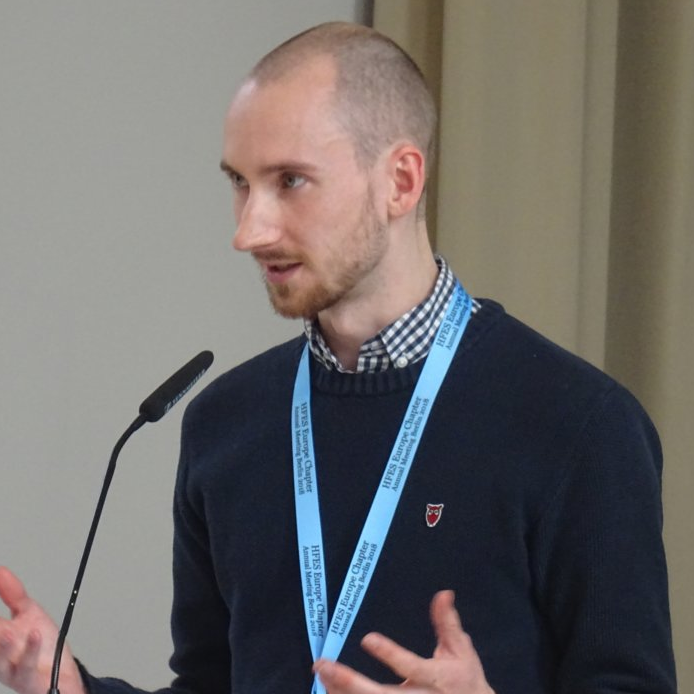
\includegraphics[width=\cvPictureWidth]{FreddySquared.png}
             };
             }]
            {};
        \end{tikzpicture}
        \end{center}

        %%%%%%%%%%%%%%%%%%%%%%%%%%%%%%%%%%%%%%%%%%%%%%%%%%%%
        % Profile section
        \ruleline{\textbf{About me}}
        I am an IT professional with a diverse background including Data Engineering and Cloud Engineering.\\ 
        I am driven by a passion to make a positive impact with technology.
        \vspace*{0.8cm} % text starts 0.4cm under the top the header

        %%%%%%%%%%%%%%%%%%%%%%%%%%%%%%%%%%%%%%%%%%%%%%%%%%%
        % Contact Section
        \ruleline{\textbf{Contact}}
        \begin{tikzpicture}[every node/.style={inner sep=0pt, outer sep=0pt}]
        \matrix [
        column 1/.style={anchor=center,contactIcon},
        column 2/.style={anchor=west,align=left,contactIcon},
        column sep=5pt,
        row sep=5pt] (contact) {
        \node{\faMale};
         & \node{Born on 29/01/1990};\\
        \node{\faEnvelope}; 
         & \node{\protect\href{mailto: f.laubisch@posteo.de}{f.laubisch@posteo.de}};\\ 
        \node{\faPhone}; 
         & \node{+49 15778944004};\\ 
        \node{\faMapMarker}; 
        & \node{Merianstr. 32A \\ 79104 Freiburg im Breisgau \\ Germany};\\
        \node{\faLinkedinSquare}; 
        & \node{\href{https://www.linkedin.com/in/frederik-laubisch/}{frederik-laubisch}};\\
        \node{\faGithub~}; 
        & \node{\protect\href{https://github.com/Kafkaese}{github.com/Kafkaese}};\\
         };
        \end{tikzpicture} 

        \vspace*{0.8cm} % text starts 0.4cm under the top the header

        %%%%%%%%%%%%%%%%%%%%%%%%%%%%%%%%%%%%%%%%%%%%%%%%%%%
        \ruleline{\textbf{Languages}}
        \begin{tikzpicture}[every node/.style={inner sep=0pt, outer sep=0pt}]
        \matrix [
        column 1/.style={anchor=center,contactIcon},
        column 2/.style={anchor=west,align=left,contactIcon},
        column sep=5pt,
        row sep=5pt] (contact) {
        \node{\flag{germany.png}};
        & \node{German - Native};\\
        \node{\flag{England.png}};
        & \node{English - Fluent};\\
        \node{\flag{France.png}};
        & \node{French - Basic};\\
        \node{\flag{arab.png}};
        & \node{Arabic - Basic};\\
        \node{\flag{Sweden.png}};
        & \node{Swedish - Basic};\\
         \node{\flag{Spain.png}};
        & \node{Spanish - Basic};\\
        };
        \end{tikzpicture} 
        
        %%%%%%%%%%%%%%%%%%%%%%%%%%%%%%%%%%%%%%%%%%%%%%%%%%%%%
        % QR Code
        %\begin{center}
        %    
\includegraphics[width=3.5cm]{QR_Info.png}
        %\end{center}
        
    \end{minipage}} %
    \hfill 
%%%%%%%%%%%%%%%%%%%%%%%%%%%%%%%%%%%%%%%%%%%%%%%%%%%%%%%%%
%%%%% MAIN SECTION %%%%%%%%%%%%%%%%%%%%
    \adjustbox{valign=t}{\begin{minipage}{13.3cm}
        \vspace*{1cm}
          
        %%%%%%%%%%%%%%%%%%%%%%%%%%%%%%%%%%%%%%%%%%%%%%%%%%%
        % Work Experience
        \section*{{\faSuitcase} WORK EXPERIENCE}


        \MySectionNoPic{2024\\ current}{Senior Data \& Cloud Engineer}{Würzburg, Germany}{\href{https://aiperia.com}{AIPERIA GmbH}}{
        \setstretch{.3}

        Joined as a Data Engineer building and maintaining ETL pipelines and customer-facing analyses, then grew into a dual role spanning both the data platform and the company's entire cloud infrastructure. Promoted to Senior in recognition of the technical ownership and leadership taken on along the way.
        
    
        \setstretch{.1}

        \begin{itemize} 
        \item Led a technical debt reduction initiative that redesigned core pipelines for scalability, cutting pipeline runtime by up to 85\% in key workflows.
        \item Established engineering best practices across the data team, including code review standards and CI/CD improvements, raising overall code quality and reliability.
        \item Modernized the development workflow: migrated dependency management to uv and introduced automated dependency updates via Renovate, reducing manual maintenance and security risk.
        \item Took on ownership of the company's AWS infrastructure as Cloud Engineer alongside Data Engineering duties — managing Kubernetes, cloud storage, monitoring/alerting, and networking.
        \item Reduced cloud storage costs by 30\% through infrastructure cleanup and optimization, while resolving significant accumulated technical debt in the platform.
        \item Regularly mentored and code-reviewed junior engineers, and served as Acting Team Lead covering for the team lead during absences.
        
        \end{itemize}}   
        
        \setstretch{.3}

        \vspace*{0.3cm}
        
        \MySectionNoPic{2023\\ current}{Portfolio Project}{Berlin, Germany}{arms-tracker.app}{Developing and maintaining \color{black}{\href{https://www.arms-tracker.app}{arms-tracker.app}, an interactive web-application visualising the flow of arms ex- and imports and the impact on global conflicts. \\
        Currently migrating deployment to new cloud provider.\\
        \href{https://github.com/Kafkaese/taro}{Github: github.com/Kafkaese/taro}} 
        }  

        

        \vspace*{0.3cm}
        
        \MySectionNoPic{2021\\ 2023}{Lead Teacher \& Batch Manager}{Berlin, Germany}{Le Wagon Berlin}{Teaching Data Science and managing the day to day operations of the Le Wagon Berlin \color{black}{\href{https://www.lewagon.com/data-science-course/full-time}{Data Science Bootcamp}}}

        \vspace*{0.3cm}

        \MySectionNoPic{2021}{Research Intern}{Berlin, Germany}{Berlin Institute of Health, Charité Berlin}{Modelling single cell RNA velocities with tools and techniques traditionally used in weather forecasting { @ \href{https://www.hidih.org/research/computational-oncology}{Computational Oncology Research Group, HiDiH}}} 
        
        %%%%%%%%%%%%%%%%%%%%%%%%%%%%%%%%%%%%%%%%%%%%%%%%%%%
        
        \section*{{\faGraduationCap} EDUCATION}

        \MySection{2020}{lelogo_bw.png}{Bootcamp}{Le Wagon Berlin}{Berlin, Germany}{Data Science}{\color{black}Final Project: \color{black!70} Authorship attribution for code using a convolutional neural network \newline
        \color{black} Github: 
        \color{black!70} \protect\href{https://github.com/jesse-lehrke/codoxer}{Codoxer}}

        \vspace*{0.30cm}
        

        \MySection{2016\\ 2019}{th.jpg}{Master of Science}{Technical University of Berlin}{Berlin, Germany}{Human Factors}{\color{black}Thesis: \color{black!70}Development and evaluation of a 3D model-based planning tool for peripheral nerve surgery in the upper extremity \newline
        \color{black} Advisor: 
        \color{black!70} \protect\href{mailto: cprahm@bgu-tuebingen.de}{Dr.scient.med. Cosima Prahm}
        \color{black} Final Grade: 
        \color{black!70} 1.8}
            
        \vspace*{0.30cm}
            
        \MySection{2010\\ 2016}{uni-osnabrueck.png}{Bachelor of Science}{University of Osnabrück}{Osnabrück, Germany}{Cognitive Science}{Thesis: \color{black!70} Extracting eye positions from electrooculographic recordings using a machine learning approach \newline
        \color{black} Advisor: 
        \color{black!70} \protect\href{mailto:krappel@uni-osnabrueck.de}{Dr.rer.nat. Kristoffer Appel} \newline
        \color{black} Final Grade: 
        \color{black!70} 1.8}
            
    \end{minipage}} %

%%%%%%%%%%%%%%%%%%%%%%%%%%%%%%%%%%%%%%%%%%%%%%%%%%%%%%%%%%%%
% Second Page
\newpage

\sidebar{sideBarColor!25}
\newpageheader{titleBackColor}{Frederik}{Laubisch}{Data Engineer | Cloud Engineer}{white}

% %%%%%%%%%%%%%%%%%%%%%%%%%%%%%%%%%% SIDEBAR %%%%%%%%%%%%%%%%%%%
\adjustbox{valign=t}{%
\begin{minipage}{5.4cm} 
\vspace*{0.4cm} % text starts 0.4cm under the top the header
        
    %%%%%%%%%%%%%%%%%%%%%%%%%%%%%%%%%%%%%%%%%%%%%%%%%%%%
    % Skill and Strengths 
    \ruleline{\textbf{Soft Skills and Strengths}}
    \vspace*{-0.5cm}
    \begin{center}
        \cvtag{Analytical Mindset}\cvtag{Critical Thinking}
        \cvtag{Sense of Responsibility}\cvtag{Problem Solving}\cvtag{Relationship Management}\cvtag{Willingness to learn} \cvtag{Ability to put complex concepts into simple terms}\cvtag{Eye for Details}\cvtag{Leadership}\cvtag{Patience}
    \end{center}

    \vspace{.4cm}

    %%%%%%%%%%%%%%%%%%%%%%%%%%%%%%%%%%%%%%%%%%%%%%%%%%%%
    % Professional Skills 
    \ruleline{\textbf{Professional Skills}}
    \begin{center}
        \cvtag{Data Sourcing} \cvtag{Web Scraping}\cvtag{Data Visualization}\cvtag{Machine Learning}\cvtag{Containerization}\cvtag{CI/CD}
    \end{center}

    \vspace{.4cm}

    %%%%%%%%%%%%%%%%%%%%%%%%%%%%%%%%%%%%%%%%%%%%%%%%%%%
    % Other Interests
    \ruleline{\textbf{Other Interests}}
    \small
    \begin{multicols}{2}
        \begin{itemize} 
            \item Bouldering \flag{mountain.png}
            \item Board Games \flag{Chess.png}
            \item Gardening \flag{Plants-Leaf-icon.png}
            \item Travels \flag{Travels.png}
            \item Books \flag{Books.png}
            \item Cooking \flag{wok.png}
            \item Democracy \flag{parliament.png}
            \item Sustainability \flag{sun.png}
    \end{itemize}
    \end{multicols}

    \vspace{.4cm}

     %%%%%%%%%%%%%%%%%%%%%%%%%%%%%%%%%%%%%%%%%%%%%%%%%%%%%
        % QR Code
        %\ruleline{\textbf{Download My CV}}
        %\scriptsize
        %\centering
        %Download my CV via the QR below \aiOverleaf.
        %\begin{center}
        %    \quad
        %    \qrcode[height=2cm]{
        %        https://www.dropbox.com/sh/k5pheguf9jrur8x%/AADpyjYJi7V5bhPyJeP3H74ea?dl=0} \\
        %    \vspace*{0.5cm}
        %\end{center}

\end{minipage}
}%
\hfill
%%%%%%%%%%%%%%%%%%%%%%%%%%%%%%%%%%% MAIN %%%%%%%%%%%%%%%%%%%%%%%%%
\adjustbox{valign=t}{%
\begin{minipage}{11.3cm}%
    \vspace*{0.4cm}%
        
    %%%%%%%%%%%%%%%%%%%%%%%%%%%%%%%%%%%%%%%%%%%%%%%%%%%
    % Information Technology Skills
    \section*{{\faDesktop} INFORMATION TECHNOLOGY SKILLS}%
    \vspace*{0.22cm}%
    \ITCcompetence{Infrastructure}{
    Docker\\
    Helm \\
    Kubernetes\\
    Terraform
    }%

    \vspace*{0.22cm}

    \ITCcompetence{Cloud}{
    AWS\\
    Azure
    }

    \vspace*{0.22cm}

    \ITCcompetence{Monitoring}{
    Grafana\\
    Loki\\
    Prometheus
    }
    
    \vspace*{0.22cm}

    \ITCcompetence{Automation}{
    Apache Airflow\\
    Github Actions\\
    Gitlab Workflows
    
    }

    \vspace*{0.22cm}

    \ITCcompetence{Data}{
    Pandas\\
    Polars\\
    SQL
    }
    
    \vspace*{0.22cm}

    \ITCcompetence{Web Development}{
    React.js\\
    HTML\\
    CSS
    }

    
    %%%%%%%%%%%%%%%%%%%%%%%%%%%%%%%%%%%%%%%%%%%%%%%%%%%
    % Programming Languages
    \section*{{\faCode} PROGRAMMING LANGUAGES}
    Python \quad\textbullet\quad SQL \quad\textbullet\quad Shell Scripting \quad\textbullet\quad JavaScript

    %%%%%%%%%%%%%%%%%%%%%%%%%%%%%%%%%%%%%%%%%%%%%%%%%%%
    % Certificates
    \section*{{\faCertificate} CERTIFICATES}
    

    \adjustbox{valign=t}{\begin{minipage}{2cm}
    \begin{center}
        
\includegraphics[width=1.4cm]{google.png}
    \end{center}
    \end{minipage}}
    \hfill \vline \hfill
    \adjustbox{valign=t}{\begin{minipage}{9cm}
        \begin{itemize}
            \scriptsize 
            \item \protect\href{https://www.coursera.org/account/accomplishments/specialization/certificate/ESUCWLJDDV6J}{Architecting with Google Compute Engine} (\textit{Coursera, 2021)} \\
            \textcolor{black}{Courses:} \color{black!70} Google Cloud Platform Fundamentals: Core Infrastructure, Essential Google Cloud  Infrastructure: Foundation, Essential Google Cloud Infrastructure: Core Services, Elastic Google Cloud Infrastructure: Scaling and Automation, Reliable Google Cloud Infrastructure: Design and Process\\
        \end{itemize}
    \end{minipage}}

\end{minipage}}


\end{document}
